\PassOptionsToPackage{expansion=false}{microtype}
\documentclass[9pt,lessons]{livecoms}
\usepackage[version=4]{mhchem}
\usepackage{siunitx}
\usepackage[italic]{mathastext}
\usepackage{amsmath,amssymb}
\usepackage{booktabs}
\usepackage{listings}
\usepackage{xcolor}
\lstset{basicstyle=\ttfamily\footnotesize, frame=single, framerule=0.4pt, rulecolor=\color{gray},
        columns=fullflexible, keepspaces=true, xleftmargin=2pt, xrightmargin=2pt, aboveskip=6pt, belowskip=6pt}
\graphicspath{{figures/}}
\newcommand{\tabdir}{tables}
\setlength{\emergencystretch}{2em}

\newcommand{\versionnumber}{0.9}
\newcommand{\githubrepository}{\url{https://github.com/sircalch/uncertainty-checks-lessons-learned}}

\title{Uncertainty and consistency checks for molecular simulation, tested on known answers and real data: MDCheck for time-series averages and FEPCert for alchemical free-energy analyses [Article v\versionnumber]}

\author[1*]{Andr\'es Monreal-Hern\'andez}
\author[2]{Sara Lizbeth Franco Amaya}
\author[3]{Carlos Ivanhoe Mart\'inez Osorio}
\affil[1]{Universidad Estatal de Sonora, Ley Federal del Trabajo s/n, 83100 Hermosillo, Sonora, Mexico}
\affil[2]{Doctorado en Nanotecnolog\'ia, Universidad de Sonora, Blvd. Luis Encinas y Rosales s/n, 83000 Hermosillo, Sonora, Mexico}
\affil[3]{Doctorado en Ciencia de Materiales, Universidad de Sonora, Blvd. Luis Encinas y Rosales s/n, 83000 Hermosillo, Sonora, Mexico}

\corr{andres.monreal@ues.mx}{AMH}

\orcid{Andr\'es Monreal-Hern\'andez}{0009-0009-1207-8597}
\orcid{Sara Lizbeth Franco Amaya}{0009-0005-0272-0241}
\orcid{Carlos Ivanhoe Mart\'inez Osorio}{0009-0003-7872-4965}

\blurb{This LiveCoMS document is maintained online on GitHub at \githubrepository; to provide feedback, suggestions, or help improve it, please visit the GitHub repository and participate via the issue tracker.}

\pubDOI{10.XXXX/YYYYYYY}
\pubvolume{<volume>}
\pubissue{<issue>}
\pubyear{<year>}
\articlenum{<number>}
\datereceived{Day Month Year}
\dateaccepted{Day Month Year}

\begin{document}

\begin{frontmatter}
\maketitle

\begin{abstract}
Uncertainty estimates and quality checks for simulated averages and free energies are rarely tested. We tested two open-source packages that automate them. MDCheck detects equilibration, reports autocorrelation-corrected confidence intervals and tests whether replicas share a mean; validated on autoregressive processes and 136 OpenMM trajectories against pymbar and pyblock. FEPCert checks overlap, TI/BAR agreement, convergence and cycle closure; it was tested on seven GROMACS legs against alchemlyb and pymbar and on the 92 maps of the FEP+ benchmark. MDCheck intervals reached nominal coverage when the effective sample size exceeded about 50, but covered only 71--79\% for 100~ps water replicas and 62--71\% for 2~ns villin observables, whose inefficiency was underestimated tenfold; a Cochran $Q$ replica test flagged them with fewer false alarms than the Gelman--Rubin rule. FEPCert matched the references to rounding error, but its earlier version passed a schedule with MBAR overlap 0.006, missed 104 of 1404 cycles and let TI deviate by 1.3--1.9~kJ\,mol$^{-1}$ where overlap passed. On the FEP+ maps, 43\% of cycles closed worse than 1.96 combined Bennett errors, against 5\% expected. A single simulation underestimates its uncertainty when shorter than its slowest relaxation; only independent replicas or estimators reveal it.
\end{abstract}

\end{frontmatter}

\section{Introduction}
Equilibrium properties are estimated from molecular dynamics (MD) simulations as time averages over a finite trajectory, and free energies as sums over a series of simulated states. Two features make the statistical error of these quantities easy to misjudge \cite{schiferl1985,straatsma1986,flyvbjerg1989error,allen2017,frenkel2002}. The simulation usually starts far from the equilibrium ensemble, so the early part of the trajectory is biased; and successive frames are correlated, so a trajectory with $N$ frames contains only $N/g$ independent samples, where $g \ge 1$ is the statistical inefficiency \cite{mullerkrumbhaar1973,sokal1997,janke2002}. Ignoring either produces error bars that are too small, sometimes by an order of magnitude. Best-practice guides therefore recommend discarding an objectively chosen equilibration period, estimating the autocorrelation time or the effective sample size, and repeating simulations from independent initial conditions \cite{grossfield2009,grossfield2018best,braun2019,knapp2018is}. For alchemical free energies, which are used routinely to rank ligands \cite{wang2015,cournia2017,mobley2017,schindler2020}, the guides add further checks \cite{pohorille2010,chodera2011,klimovich2015,mey2020}: neighbouring states must overlap in phase space (quantified with the MBAR overlap matrix and a threshold of 0.03 \cite{klimovich2015}); TI must use enough states where $\langle \partial H/\partial\lambda\rangle$ is curved \cite{paliwal2011,bruckner2011}; the estimate must not drift with simulation time \cite{klimovich2015,chodera2016}; and in a network of relative free energies the sum around every thermodynamic cycle should vanish within its statistical error \cite{wang2013,wang2015,hahn2022}.

Each step has a mature methodological literature. Block averaging \cite{flyvbjerg1989error,lee2011} and windowed estimators of the integrated autocorrelation time \cite{madras1988,sokal1997,geyer1992,wolff2004} estimate $g$; several rules truncate initialisation bias, from reverse cumulative averaging \cite{yang2004} and the marginal standard error rule \cite{white1997} to the maximisation of the effective sample size \cite{chodera2016simple}; independent replicas are advocated as the most reliable route to uncertainty quantification \cite{coveney2016,bhati2017,wan2021}; and in Markov chain Monte Carlo the equivalent task is solved with the Gelman--Rubin factor $\hat{R}$ \cite{gelman1992,brooks1998,vehtari2021}. Robust implementations of individual steps exist: pymbar \cite{shirts2008mbar,chodera2016simple}, pyblock \cite{lee2011}, alchemlyb \cite{wu2024alchemlyb,klimovich2015,mey2020,wu2024}, MDAnalysis \cite{michaud2011} and ArviZ \cite{kumar2019}. In practice, however, the steps are applied inconsistently, if at all, and rarely reported in a form that a reader can check; and it is uncommon for a tool to document the property that matters to the user, namely whether its nominal 95\% interval contains the ensemble average in 95\% of cases.

The first author wrote two open-source Python packages that apply these steps uniformly and write a report with a draft methods paragraph: MDCheck, for scalar time series from GROMACS, LAMMPS, OpenMM, AMBER and NAMD, and FEPCert, for GROMACS free-energy output or tables of gradients, work values and network edges. This article reports how well they work, measured on processes with known answers and on real data, with independent implementations as references. The validation changed both packages: it exposed an interval in MDCheck 1.0.0 that was systematically too narrow and a replica criterion that raised alarms for replicas of the same ensemble, and it exposed an ``overlap'' in FEPCert that did not measure overlap, a cycle enumeration that missed 7\% of the cycles and thresholds that ignored the energy unit. The defects are reported together with their corrections (MDCheck 1.1.0, FEPCert 1.2.0). The validation also identifies the regime in which no single-trajectory estimate can deliver nominal coverage, and shows that a calibrated replica test detects it.

\section{Methods implemented}

\subsection{MDCheck}
Figure~\ref{fig:mdwf} summarises the analysis applied to each observable, a scalar time series $x_1,\dots,x_N$ sampled at a constant interval.

\begin{figure*}[t]
\centering
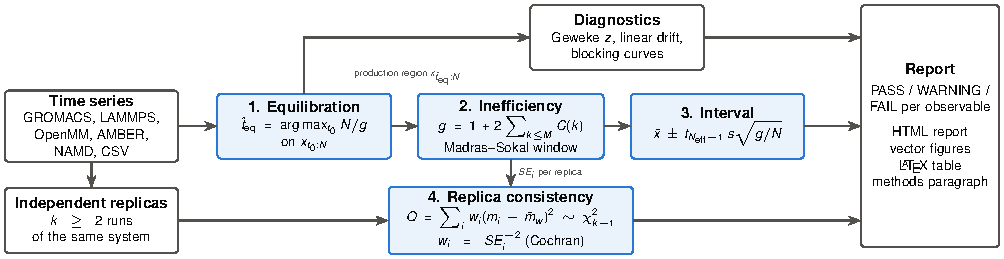
\includegraphics[width=\textwidth]{mdcheck_workflow.pdf}
\caption{Analysis performed by MDCheck for each observable. The equilibration time is chosen by maximising the effective sample size of the retained production region. The statistical inefficiency of that region defines the confidence interval of its mean. Autocorrelation-corrected standard errors of independent replicas feed a heterogeneity test. Stationarity and drift diagnostics are reported alongside but do not change the interval.}
\label{fig:mdwf}
\end{figure*}

\paragraph{Autocorrelation and statistical inefficiency.}
The normalised autocorrelation function
\begin{equation}
C(k) = \frac{1}{(N-k)\,\hat\sigma^2}\sum_{i=1}^{N-k}(x_i-\bar x)(x_{i+k}-\bar x), \qquad \hat\sigma^2 = \frac{1}{N}\sum_{i=1}^{N}(x_i-\bar x)^2,
\end{equation}
is computed by fast Fourier transform. The integrated autocorrelation time is estimated with the self-consistent window of Madras and Sokal \cite{madras1988,sokal1997},
\begin{equation}
\hat\tau_{\mathrm{int}} = \tfrac12 + \sum_{k=1}^{M} C(k), \qquad M = \min\{k : k \ge c\,\hat\tau_{\mathrm{int}}(k)\ \text{or}\ C(k) < 0\},
\end{equation}
with $c = 6$. The statistical inefficiency and effective sample size are
\begin{equation}
g = 2\hat\tau_{\mathrm{int}} = 1 + 2\sum_{k=1}^{M} C(k), \qquad N_{\mathrm{eff}} = N/g .
\end{equation}

\paragraph{Equilibration detection.}
Following Chodera \cite{chodera2016simple}, the equilibration time is the cutoff that maximises the effective size of the retained production region,
\begin{equation}
\hat t_{\mathrm{eq}} = \arg\max_{0 \le t_0 \le 0.85N} \frac{N - t_0}{g(x_{t_0+1:N})}.
\end{equation}
Evaluating $g$ is $O(N\log N)$, so an exhaustive search is quadratic in $N$. MDCheck evaluates the objective on a grid of stride $s_0=\max(10, \lfloor N/200\rfloor)$ and refines the grid hierarchically around the current optimum with strides $s_0/10, s_0/100,\dots$ down to one sample, which takes about 250 evaluations independently of $N$.

\paragraph{Confidence interval of the production mean.}
The 95\% confidence interval of the production mean is
\begin{equation}
\bar x \pm t_{0.975,\,N_{\mathrm{eff}}-1}\; s\sqrt{g/N_{\mathrm{prod}}},
\label{eq:ci}
\end{equation}
where $s$ is the sample standard deviation of the production region; the Student-$t$ quantile \cite{student1908} widens the interval for short series. Version 1.0.0 instead reported a moving-block bootstrap interval \cite{kunsch1989} with blocks of length $\lceil 2\hat\tau_{\mathrm{int}}\rceil$.

\paragraph{Consistency between replicas.}
For $k$ independent replicas with production means $m_i$ and autocorrelation-corrected standard errors $SE_i = s_i\sqrt{g_i/n_i}$, MDCheck computes Cochran's heterogeneity statistic \cite{cochran1954}
\begin{equation}
Q = \sum_{i=1}^{k} w_i (m_i - \bar{m}_w)^2,\qquad w_i = SE_i^{-2},\qquad \bar{m}_w = \frac{\sum_i w_i m_i}{\sum_i w_i}.
\end{equation}
When all replicas sample the same ensemble and the standard errors are correct, $Q$ follows a $\chi^2_{k-1}$ distribution. The status is PASS for $p \ge 0.05$, WARNING for $0.01 \le p < 0.05$ and FAIL for $p < 0.01$, so the nominal false-alarm rate is fixed by these levels; the fraction of variation attributable to heterogeneity, $I^2 = \max(0, (Q-k+1)/Q)$ \cite{higgins2002}, is reported alongside, and Jensen--Shannon \cite{lin1991}, Kolmogorov--Smirnov and Wasserstein distances between replica histograms are reported as descriptors only. In version 1.0.0 the status was decided by a Jensen--Shannon distance threshold of 0.15.

\paragraph{Stationarity diagnostics and implementation.}
Geweke's $z$ score \cite{geweke1992} (first 10\% against last 50\% of the production region, with autocorrelation-corrected variances) and a linear drift of the production mean are reported without changing the interval, and Flyvbjerg--Petersen blocking curves \cite{flyvbjerg1989error} are plotted for inspection. An observable is flagged FAIL when $N_{\mathrm{eff}} < 100$ and WARNING when $N_{\mathrm{eff}} < 500$ (configurable). MDCheck is pure Python ($\ge 3.9$), depends on NumPy \cite{harris2020}, SciPy \cite{virtanen2020}, pandas \cite{mckinney2010}, Matplotlib \cite{hunter2007} and Jinja2, is distributed under the MIT licence, and reads GROMACS \texttt{.xvg} files \cite{abraham2015}, LAMMPS thermo output \cite{thompson2022}, OpenMM \texttt{StateDataReporter} logs \cite{eastman2024openmm}, AMBER \texttt{cpptraj} files \cite{case2005}, NAMD output \cite{phillips2020} and generic delimited text. A complete analysis is one command,
\begin{lstlisting}
mdcheck assess -i energy.xvg -o report/
\end{lstlisting}
and each analysis writes an HTML report, vector figures, a \LaTeX{} summary table and a draft methods paragraph that states the settings used.

\subsection{FEPCert}
Figure~\ref{fig:fepwf} summarises what FEPCert computes.

\begin{figure*}[t]
\centering
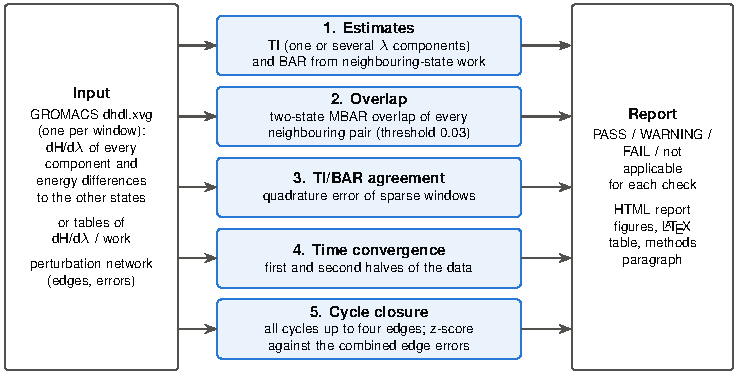
\includegraphics[width=\textwidth]{fepcert_workflow.pdf}
\caption{FEPCert workflow. Each check returns PASS, WARNING, FAIL or, when the input does not determine it, not applicable.}
\label{fig:fepwf}
\end{figure*}

\paragraph{Estimates.}
TI integrates $\langle \partial H/\partial\lambda\rangle$ by the trapezoidal rule. When several lambda components change along one set of windows, as in GROMACS absolute binding free energies (restraints, Coulomb and van der Waals), the windows are ordered by the sum of their lambda values and each component is integrated over its own lambda; the standard error of each window mean is corrected for autocorrelation by the statistical inefficiency, and the variances are propagated through the quadrature weights. BAR is solved self-consistently for each pair of neighbouring states, with the asymptotic variance of Shirts et al.\ \cite{shirts2003}. For GROMACS files, the energy differences to the other states written in each dhdl.xvg file provide the forward work $W_\mathrm{F} = H_{k+1} - H_k$ on samples of state $k$ and the reverse work $W_\mathrm{R} = H_k - H_{k+1}$ on samples of state $k+1$.

\paragraph{Checks.}
\emph{Overlap}: for each neighbouring pair, the MBAR weights of the two states \cite{shirts2008} are computed from the reduced work values and the overlap is $O_{01} = N_1 \sum_n W_{n0} W_{n1}$, the off-diagonal element of the overlap matrix of Klimovich et al.\ \cite{klimovich2015} restricted to the pair; the smallest overlap passes above 0.08, warns between 0.03 and 0.08 and fails below 0.03, and when only dH/d$\lambda$ is available the check is reported as not applicable, because the distribution of dH/d$\lambda$ does not determine phase-space overlap. \emph{TI/BAR agreement}: trapezoidal TI carries a quadrature error where the states are too sparse for the curvature of $\langle \partial H/\partial\lambda\rangle$, and BAR on the same states does not; a difference larger than three combined standard errors and than 0.25~kcal\,mol$^{-1}$ warns, and larger than 1~kcal\,mol$^{-1}$ fails. \emph{Time convergence}: TI estimates from the first and second halves of the data are compared (pass below 0.4~kcal\,mol$^{-1}$, warning below 0.8) and forward and backward estimates from growing fractions of the data are reported; all thresholds are defined in kcal\,mol$^{-1}$ and converted when the data are in kJ\,mol$^{-1}$. \emph{Cycle closure}: every simple cycle of up to four edges of the perturbation graph is enumerated, each identified by its set of edges; its closure error is the signed sum of the edge free energies, and with edge uncertainties $\sigma_e$ the cycle has an expected spread $\sigma_c = (\sum_e \sigma_e^2)^{1/2}$ and a z-score $z = \text{closure}/\sigma_c$.

\section{Validation design}

\subsection{MDCheck: processes with known answers}
First-order autoregressive processes, AR(1), $x_t = \phi x_{t-1} + \varepsilon_t$, with unit marginal variance have mean zero and exact statistical inefficiency $g = (1+\phi)/(1-\phi)$. Three sets of series were used. (1)~\emph{Inefficiency and coverage}: for $\phi \in \{0, 0.5, 0.8, 0.9, 0.95, 0.99\}$ ($g$ from 1 to 199), 100 series of $N = 20\,000$ samples each, and five 95\% intervals for the mean: the naive interval $\bar{x} \pm 1.96\,s/\sqrt{N}$, the version 1.0.0 block bootstrap, the version 1.1.0 interval of Eq.~(\ref{eq:ci}), the same interval with $g$ from pymbar's \texttt{statistical\_inefficiency}, and pyblock's standard error at its optimal block size. (2)~\emph{Series length and window constant}: for $\phi \in \{0.5, 0.9, 0.95\}$ and $N$ from 250 to 20\,000 (500 series each), the naive interval, a normal-quantile interval with estimated $g$, and Eq.~(\ref{eq:ci}) with $c \in \{4, 6, 8\}$. (3)~\emph{Equilibration}: an offset $5\,e^{-t/\tau_{\mathrm{relax}}}$ was added to AR(1) series ($\phi = 0.9$, $\tau_{\mathrm{relax}} = 300$; $\phi = 0.95$, $\tau_{\mathrm{relax}} = 1000$; $N = 10\,000$; 25 series each), and the equilibration time and residual bias were compared with \texttt{pymbar.timeseries.detect\_equilibration}.

\subsection{MDCheck: molecular dynamics}
All simulations used OpenMM 8.6.1 \cite{eastman2024openmm} with the Langevin middle integrator \cite{zhang2019} and a friction of 1~ps$^{-1}$, on the OpenCL platform. \emph{Lennard-Jones argon}: 864 atoms ($\sigma = 3.405$~\AA, $\varepsilon/k_B = 119.8$~K, $m = 39.948$~u) at reduced density $\rho^* = 0.8442$ and $T = 94.4$~K ($T^* = 0.788$) \cite{verlet1967}, cutoff $3\sigma$ with the long-range dispersion correction, 10~fs time step, potential energy sampled every 0.25~ps; every run started from an fcc lattice, so each replica contains a genuine melting transient (Fig.~\ref{fig:length}b). \emph{TIP3P water}: a 3~nm cubic box of 887 TIP3P molecules \cite{jorgensen1983} with particle-mesh Ewald electrostatics \cite{essmann1995} and a 0.9~nm cutoff, rigid water, a 2~fs time step and a Monte Carlo barostat \cite{aqvist2004} at 1~bar and 300~K, velocities initialised at 200~K, potential energy and density sampled every 0.2~ps. \emph{Villin headpiece}: the folded 35-residue HP35 solvated in 2761 TIP3P molecules (8867 atoms), distributed with OpenMM as \texttt{test.pdb}, with the Amber14 force field \cite{maier2015ff14sb}, PME with a 0.9~nm cutoff, constraints on bonds to hydrogen, hydrogen mass repartitioning to 4~u \cite{hopkins2015}, a 4~fs time step and a Monte Carlo barostat at 1~bar and 300~K, velocities drawn at 300~K; the C$\alpha$ root-mean-square deviation (RMSD) from the starting structure, the radius of gyration $R_g$ and the potential energy were sampled every 5~ps, adding observables whose relaxation is slow compared with a short replica.

For each system, four long reference runs define the reference mean and its standard error from the spread of the run means: for argon 1500~ps with the first 100~ps discarded, for water 600~ps with 50~ps discarded, for villin four runs of 15~ns with the first 2~ns discarded. Independent short replicas were then analysed exactly as a user would analyse them: 48 replicas of 150~ps for argon; for water 24 replicas of 100~ps and, in a separate campaign, 24 of 300~ps with 1200~ps reference runs; for villin 24 replicas of 2~ns. A replica interval was counted as covering the reference if $|\bar{x} - \mu_{\mathrm{ref}}| \le t\,\sqrt{SE^2 + SE_{\mathrm{ref}}^2}$, so that the uncertainty of the reference does not count against the method. Random triples of replicas of the same ensemble (400 per data set) measured how often each replica criterion raises a false alarm; to measure power, a shift of $k \in \{1,2,3,4,6\}$ standard errors was added to one replica of each triple, using that replica's own autocorrelation-corrected standard error, so that the noise is genuine MD noise and only the mean differs. The $Q$ test was compared with the rank-normalised split $\hat{R}$ of ArviZ \cite{vehtari2021,kumar2019} at the thresholds 1.01 \cite{vehtari2021} and 1.1 \cite{gelman1992,brooks1998}, and with the Jensen--Shannon criterion of version 1.0.0. The reference implementations were pymbar 4.0.3, pyblock and ArviZ 1.3.0, and seeds are fixed in every script.

\subsection{FEPCert: GROMACS data and the FEP+ benchmark}
The alchemtest collection provides the dhdl.xvg files of several GROMACS calculations: the hydration free energies of benzene and ethanol, each in a Coulomb leg and a van der Waals leg; the ligand and complex legs of the absolute binding free energy of $n$-phenylglycinonitrile to T4 lysozyme, in which restraints \cite{boresch2003}, Coulomb and van der Waals interactions change along 20 and 30 states; and a water particle between two surfaces with Coulomb and van der Waals components along 38 states. Each of the seven legs was analysed with all states and samples (\emph{full}), with the first 5\% of the samples of every state (\emph{short}), and with every second (\emph{sparse}) or every fourth state (\emph{very sparse}), keeping both end states, giving 28 analyses. The references were alchemlyb 2.5 \cite{wu2024} (TI, BAR, forward/backward convergence) and pymbar 4 \cite{shirts2008} (two-state and multi-state MBAR overlap); FEPCert 1.1.0 was applied to the same data for comparison. The public FEP+ benchmark \cite{ross2023} provides, for every edge of 92 perturbation maps, the Bennett free energy and its standard error; cycles of up to four edges were enumerated independently with networkx, and FEPCert 1.1.0 and 1.2 were applied to the same edges.

\section{Results}

\subsection{MDCheck: statistical inefficiency and interval coverage}\label{sec:ar1}
MDCheck's estimate of $g$ agreed with the exact value over two orders of magnitude and with pymbar's estimate (Fig.~\ref{fig:ar1}a, Table~\ref{tab:ar1}); both show the expected growth of scatter with $g$ at fixed $N$. The naive standard error lost coverage steadily as correlation increased, down to 0.09 at $\phi = 0.99$ (Fig.~\ref{fig:ar1}b). The version 1.0.0 block-bootstrap interval stayed between 0.82 and 0.90 for $\phi \ge 0.5$; its half-width was 75--81\% of the exact value, because blocks of length $2\hat\tau_{\mathrm{int}}$ are too short to capture the tail of the correlation \cite{kunsch1989,politis1994}. Eq.~(\ref{eq:ci}), the interval with pymbar's $g$, and pyblock all gave coverage between 0.90 and 0.99, consistent with the nominal 0.95 within the Monte Carlo uncertainty of $\pm 0.04$ for 100 series.

\begin{figure*}[t]
\centering
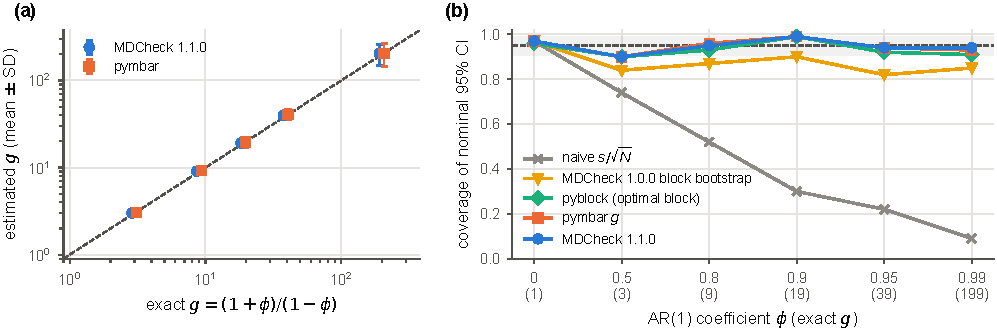
\includegraphics[width=\textwidth]{fig2_ar1.pdf}
\caption{AR(1) benchmark ($N = 20\,000$, 100 series per $\phi$). (a) Statistical inefficiency estimated by MDCheck and pymbar against the exact value (mean $\pm$ SD). (b) Coverage of nominal 95\% intervals for the true mean. The dashed line marks 0.95, and the shaded band is the 95\% Monte Carlo range for 100 series.}
\label{fig:ar1}
\end{figure*}

\begin{table*}[t]
\centering\small
\caption{AR(1) benchmark: statistical inefficiency and coverage of nominal 95\% intervals for the true mean (100 series of $N = 20\,000$ per $\phi$).}
\label{tab:ar1}
\resizebox{\textwidth}{!}{\input{\tabdir/table_ar1.tex}}
\end{table*}

Coverage of Eq.~(\ref{eq:ci}) was nominal whenever the true effective sample size $N/g$ exceeded about 50, for all three correlation levels (Fig.~\ref{fig:length}a; Table~S2 in the Supplementary Information). Below that it fell to 0.87--0.93, reaching its minimum at $N/g \approx 6$, because windowed autocorrelation estimators are biased downwards in short series: at $\phi = 0.95$ and $N = 250$ the median estimate of $g$ was 23.6 instead of 39. The Student-$t$ quantile recovered part of the loss (coverage rose from 0.84 to 0.87 at $N/g \approx 6$), and the window constant had almost no effect: coverage with $c = 4$, 6 and 8 differed by at most 0.01. The default thresholds of MDCheck (FAIL below $N_{\mathrm{eff}}=100$, WARNING below 500) are therefore conservative relative to the validity of the interval.

\begin{figure*}[t]
\centering
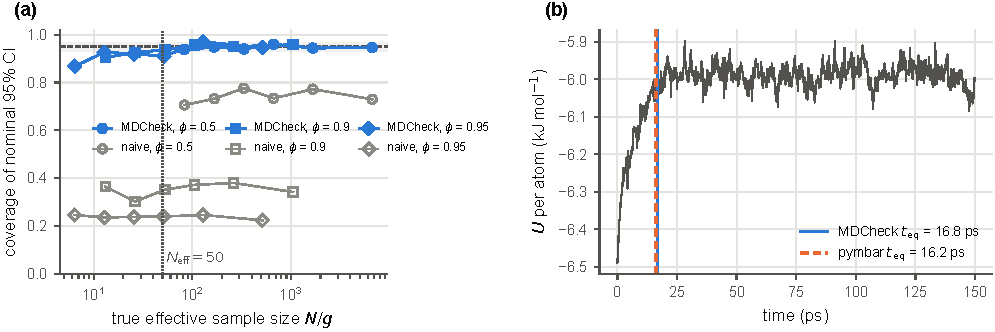
\includegraphics[width=\textwidth]{fig3_length_trace.pdf}
\caption{(a) Coverage of the MDCheck interval and of the naive interval against the true effective sample size for AR(1) processes (500 series per point). The dotted line marks $N/g = 50$. (b) Potential energy per atom of one Lennard-Jones replica started from an fcc lattice, with the equilibration times chosen by MDCheck and pymbar.}
\label{fig:length}
\end{figure*}

\subsection{MDCheck: equilibration detection and computational cost}
On AR(1) series with an initial transient, MDCheck and pymbar chose equilibration times that differed by a median of 1 and 2 samples (Table~\ref{tab:eq}), as expected since both maximise $N_{\mathrm{eff}}$; discarding the detected transient reduced the bias of the mean from 0.150 to 0.016 and from 0.495 to 0.077, in units of the marginal standard deviation. In the argon replicas the median equilibration times were 15.2~ps (MDCheck) and 16.2~ps (pymbar); Fig.~\ref{fig:length}b shows a representative melting transient. The hierarchical search returned the same equilibration time as the exhaustive stride-10 search of version 1.0.0 for all 120 argon and water replicas; for $N = 10^4$ it took 0.40~s, against 1.79~s for the exhaustive search and 3.22~s for pymbar's exact search, and for $N = 10^6$ it took 122~s, against 216~s for pymbar's \texttt{fast} mode, which resolves $t_{\mathrm{eq}}$ only to its stride of $N/200$ samples (Table~S3).

\begin{table*}[t]
\centering\small
\caption{Equilibration detection on AR(1) series with an exponential initial transient (25 series each). The bias is in units of the marginal standard deviation.}
\label{tab:eq}
\input{\tabdir/table_equilibration.tex}
\end{table*}

\subsection{MDCheck: coverage on OpenMM trajectories}
Table~\ref{tab:md} and Fig.~\ref{fig:md}a summarise the MD benchmark. For argon, keeping the melting transient would have biased the mean by $-7.1$ standard errors. MDCheck's interval covered the reference mean in 90\% of the 48 replicas, and in 94\% after a further 20~ps discard; the residual shortfall is consistent with the known tendency of the maximum-$N_{\mathrm{eff}}$ rule to cut slightly early, trading a small bias for variance \cite{chodera2016simple}. With the naive standard error, coverage was 0.65.

For water, coverage with 100~ps replicas was 0.79 for density and 0.71 for potential energy, well above the naive 0.21--0.29 but below nominal, and a further discard did not help. The cause is the inefficiency estimate, not the equilibration cutoff: the median $g$ from 100~ps replicas (9.5--10.0) was about 30\% smaller than the value obtained from the 600~ps reference runs (about 14), because a slow, low-amplitude tail of the autocorrelation cannot be resolved in a short series. Any estimator that uses only the series itself inherits this limitation; on the same production segments, the Madras--Sokal window, truncation at the first negative autocorrelation, Geyer's initial monotone sequence \cite{geyer1992} and pymbar gave identical coverage and inefficiencies within 4\% (Table~S1). With 300~ps replicas the median $g$ rose to 10.7--10.9 and $N_{\mathrm{eff}}$ tripled; coverage then recovered to 0.96 for density and 0.92 for potential energy (0.96 with a further 20~ps discard), while the naive interval still covered only 0.42--0.67 of replicas.

Villin shows the limit of any single-trajectory estimate. For the potential energy, which decorrelates within one sample ($g = 1.2$), MDCheck and the naive interval both covered 0.83 of the replicas, and 0.92 after a further 200~ps discard. For $R_g$ and the C$\alpha$ RMSD, the replicas detected equilibration times near 0.9~ns (median per-replica difference from pymbar 12.5 and 57.5~ps) and kept only 19--26 effective samples. The median $g$ of the 2~ns replicas was 9.8--10.3, whereas the 15~ns reference runs gave 101--117 for the same observables: the slow conformational relaxation is invisible within 2~ns, so the intervals were too narrow. Coverage was 0.62 for $R_g$ and 0.71 for the RMSD, against 0.50--0.54 for the naive interval, and a further discard did not help; keeping the initial relaxation gave wider intervals and higher coverage but biased the mean by $-1.2$ and $-2.0$ standard errors, so it is not a remedy.

\begin{table*}[t]
\centering\scriptsize
\caption{OpenMM benchmark. For each data set: median equilibration time, statistical inefficiency and $N_{\mathrm{eff}}$; coverage of the reference mean by the naive interval, by MDCheck, and by MDCheck with a further discard (20~ps; 200~ps for villin); bias of the mean without any equilibration discard, in production standard errors; and alarm rates of the replica tests on non-overlapping triples of replicas of the same ensemble (nominal 0.05 for the $Q$ test).}
\label{tab:md}
\resizebox{\textwidth}{!}{\input{\tabdir/table_md.tex}}
\end{table*}

\begin{figure*}[t]
\centering
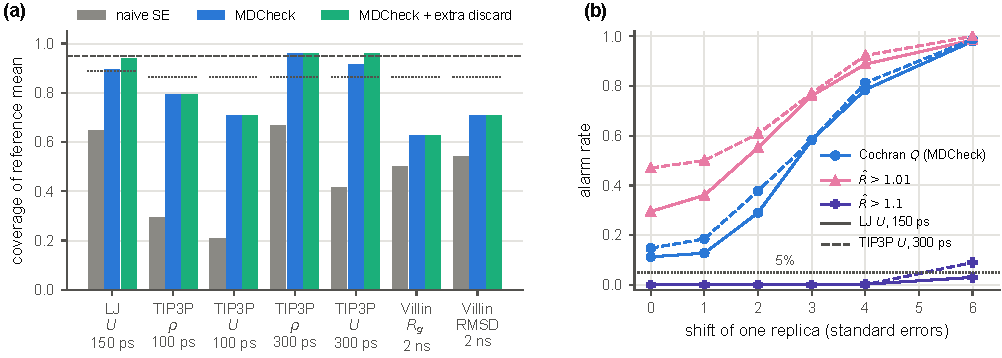
\includegraphics[width=\textwidth]{fig4_md.pdf}
\caption{(a) Coverage of the reference mean for OpenMM replicas; the extra discard is 20~ps (200~ps for villin). Dotted lines mark the lower 95\% Monte Carlo limit for the number of replicas. (b) Alarm rate of replica-consistency criteria for random triples of replicas when one replica is shifted by a given number of its standard errors (400 triples per point). Solid lines: Lennard-Jones potential energy; dashed lines: TIP3P potential energy, 300~ps replicas.}
\label{fig:md}
\end{figure*}

\subsection{MDCheck: replica-consistency tests}
Replicas of the same ensemble should rarely fail a consistency check, and a displaced replica should be detected (Fig.~\ref{fig:md}b, Table~\ref{tab:rep}). The Jensen--Shannon criterion of version 1.0.0 fails the first requirement: it raised an alarm for every triple in the argon and 100~ps water sets, and for 29--32\% of triples at 300~ps, because histogram divergences between finite, autocorrelated samples are biased upwards and depend on sample size. The $\hat{R} > 1.01$ threshold recommended for MCMC \cite{vehtari2021} behaved similarly, with false alarms in 19--47\% of triples for argon and 300~ps water and in 88--92\% for 100~ps water, because it assumes thousands of effective draws per chain, far more than a typical MD replica provides; the classical threshold $\hat{R} > 1.1$ \cite{gelman1992,brooks1998} almost never raised an alarm for argon and 300~ps water, even when one replica was displaced by six standard errors (0--9\%).

The $Q$ test combined low false-alarm rates with useful power. Without a shift it raised alarms in 3--15\% of triples for argon and 300~ps water; with a shift of three standard errors it detected 58--61\% of the displaced triples, and with six standard errors 98--99\%. Its false-alarm rate exceeded the nominal 5\% where the per-replica standard errors were underestimated (28--29\% for 100~ps water, and 11\% for argon, where coverage was 0.90), so the replica test is the check that detects underestimated single-trajectory uncertainties. The villin replicas have no injected shift, but they do not share a mean within their standard errors, so an alarm there is a correct detection: the $Q$ test raised alarms in 82--87\% of random triples (75--100\% of non-overlapping triples; Table~\ref{tab:md}), and $\hat{R} > 1.1$ in 91--92\% (median $\hat{R}$ 1.32--1.40). All criteria agree that 2~ns replicas cannot resolve these observables, which is the situation in which the single-trajectory intervals were too narrow.

\begin{table*}[t]
\centering\small
\caption{Alarm rates of replica-consistency criteria for random triples of replicas (400 per entry), without and with a shift of one replica by 3 or 6 of its standard errors (SE). The villin replicas are not converged at 2~ns, so alarms without an injected shift are correct detections, not false alarms.}
\label{tab:rep}
\resizebox{\textwidth}{!}{\input{\tabdir/table_replica_tests.tex}}
\end{table*}

\subsection{MDCheck: defects found by the validation}
Two defects of version 1.0.0 were invisible to unit tests and appeared only when coverage and false-alarm rates were measured on data with a known answer: the block-bootstrap interval, which covered the true mean in 82--90\% of cases, and the fixed Jensen--Shannon threshold, which raised an alarm for every group of replicas drawn from the same ensemble. Both are replaced in version 1.1.0. The validation also corrected two parser defects (an incompatibility with pandas~3 in the AMBER reader, and loss of the column names written by \texttt{cpptraj}), and a LAMMPS reader announced in earlier documentation but not implemented was added.

\subsection{FEPCert: agreement with the reference implementations}
Every estimate agreed with its reference to rounding error (Table~\ref{tab:agree}). This includes TI along the multi-component paths of the binding free energy and the water particle (complex leg 90.018~kJ\,mol$^{-1}$, ligand leg 32.535~kJ\,mol$^{-1}$), which version 1.1.0 rejected, and BAR from the energy differences read directly from the GROMACS files. The two-state overlap agreed with pymbar to $4\times10^{-12}$. The standard errors of TI were 0.72--0.98 times those of alchemlyb after decorrelation (median 0.80); both correct for autocorrelation, FEPCert through the statistical inefficiency of all samples and alchemlyb by subsampling, and the difference reflects their estimates of the correlation time.

\begin{table*}[t]
\centering\small
\caption{Agreement of FEPCert 1.2 with independent implementations.}
\label{tab:agree}
\resizebox{\textwidth}{!}{\input{\tabdir/table_agreement.tex}}
\end{table*}

\subsection{FEPCert: overlap}
Version 1.1.0 computed its ``overlap'' from histograms of dH/d$\lambda$ in neighbouring states and compared it with the threshold of Klimovich et al. On the 16 single-component analyses it passed 15 and warned once, and its ranking of neighbouring pairs was unrelated to the MBAR overlap (Spearman correlations between $-0.58$ and 1.0; Fig.~\ref{fig:overlap}a); in particular, it passed the very sparse ethanol van der Waals leg with a value of 0.15, whereas the MBAR overlap of its worst pair was 0.006. The two-state MBAR overlap of version 1.2 followed the multi-state MBAR overlap wherever overlap was poor, and failed exactly the three analyses in which the multi-state overlap fell below 0.03. For well-overlapping states it is larger than the multi-state value, because each state shares weight with fewer neighbours, so the threshold is the more conservative where it matters.

\begin{figure*}[t]
\centering
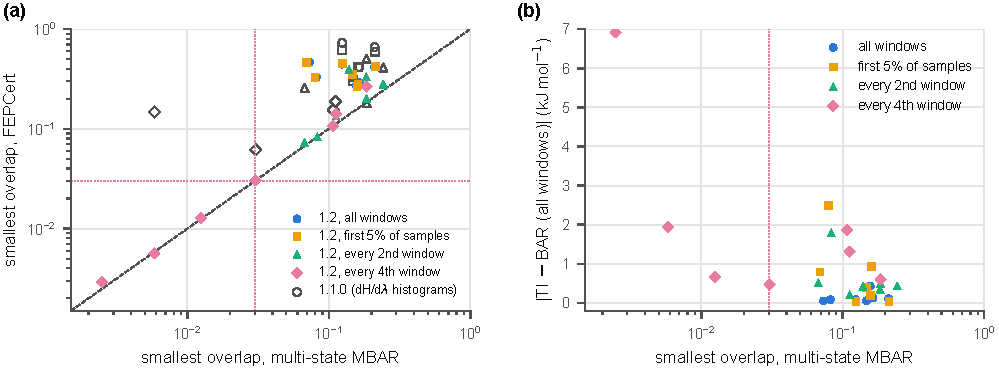
\includegraphics[width=\textwidth]{fig2_overlap.pdf}
\caption{Overlap and quadrature error on 28 GROMACS analyses (7 legs, 4 lambda schedules). (a) Smallest neighbouring-state overlap reported by FEPCert against the multi-state MBAR overlap (pymbar); filled symbols, version 1.2 (two-state MBAR); open symbols, version 1.1.0 (dH/d$\lambda$ histograms, single-component legs only). Dotted lines, 0.03. (b) Deviation of TI from BAR with all states against the multi-state overlap.}
\label{fig:overlap}
\end{figure*}

\subsection{FEPCert: quadrature error, time convergence and units}
Overlap protects BAR and MBAR, but TI fails differently. With every fourth state, TI deviated from the full-schedule BAR value by 0.5--6.9~kJ\,mol$^{-1}$ (Fig.~\ref{fig:overlap}b), while BAR on the same thinned states stayed within 0.4~kJ\,mol$^{-1}$. In two of these analyses (the Coulomb legs of benzene and ethanol, deviations of 1.9 and 1.3~kJ\,mol$^{-1}$) the overlap was still above 0.1 and passed; the TI/BAR agreement check flagged them, with differences of 14 and 7 combined standard errors, as well as the ethanol van der Waals and ligand legs, and raised no warning in the 21 full, short and sparse analyses (Table~S6). Every very sparse analysis in which TI deviated by more than 0.7~kJ\,mol$^{-1}$ was flagged by the overlap, the TI/BAR check or both, so a TI estimate should be accompanied by BAR or MBAR on the same states whenever the energy differences are available.

The forward and backward estimates of FEPCert agreed with alchemlyb's to $10^{-13}$~kJ\,mol$^{-1}$. Version 1.1.0 applied its kcal\,mol$^{-1}$ thresholds to values in kJ\,mol$^{-1}$; on the short analyses it failed benzene's van der Waals leg and warned on both ethanol legs, although the two halves of the data differed by only 0.27--0.83~kJ\,mol$^{-1}$ (0.06--0.20~kcal\,mol$^{-1}$), well inside the uncertainty. Version 1.2 passes them. Through the command line, which converts GROMACS energies to kcal\,mol$^{-1}$ by default, the defect appeared only when results were requested in kJ\,mol$^{-1}$; through the programming interface it applied to any kJ\,mol$^{-1}$ input, and it also affected the TI and BAR error thresholds.

\subsection{FEPCert: cycle closure in the FEP+ benchmark}
The 92 maps contain 1404 cycles of three or four edges (510 triangles and 894 four-edge cycles). Version 1.1.0 identified four-edge cycles by their four ligands, so that the distinct cycles through the same four ligands collapsed into one; it found 1300 cycles and missed 104 in 18 maps (Fig.~\ref{fig:cycles}a). Its network-level verdicts did not change, but its largest closure error was underestimated in several maps, for example 1.25 instead of 1.74~kcal\,mol$^{-1}$ for TYK2. Version 1.2 finds all 1404 cycles, with closure statistics identical to the networkx enumeration.

The z-scores show a more general problem (Fig.~\ref{fig:cycles}b). If the Bennett standard errors of the edges described the actual uncertainty, about 5\% of the cycles would close worse than 1.96 combined errors and the median $|z|$ would be 0.67. In the 1399 cycles with reported errors, 43\% exceeded 1.96, 24\% exceeded 3, and the median $|z|$ was 1.65; the distribution is matched closely by inflating every edge error by a factor of 2.5. The cycles share edges and are not independent, but the excess was present in all 13 groups of maps (33--80\% beyond 1.96, apart from one group of four maps with 23\%). This agrees with the observation that analytical BAR errors, which treat the samples of one simulation as the only source of variance, underestimate the spread of repeated calculations \cite{bhati2018,wan2020}, and it is why cycle-closure-based errors are preferred for networks \cite{wang2013,wang2015}. FEPCert therefore reports the z-scores, so that a network whose closures exceed their stated errors is not accepted on the closure RMSE alone.

\begin{figure*}[t]
\centering
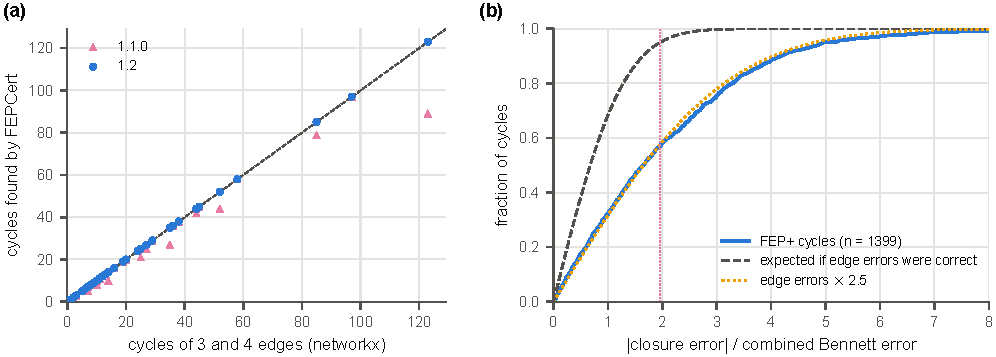
\includegraphics[width=\textwidth]{fig3_cycles.pdf}
\caption{Cycle closure in the 92 maps of the public FEP+ benchmark. (a) Number of cycles of three and four edges found by FEPCert against networkx. (b) Cumulative distribution of the closure error divided by the combined Bennett error of the cycle; dashed, the half-normal distribution expected if the edge errors were correct; dotted, the same with all edge errors multiplied by 2.5.}
\label{fig:cycles}
\end{figure*}

\subsection{What the two tests have in common}
Three lessons recur. First, \emph{the uncertainty of one simulation is underestimated when the simulation is shorter than the slowest relaxation it samples}: the 100~ps water and 2~ns villin intervals of MDCheck were too narrow because the slow tail of the autocorrelation function was not in the series, and the Bennett errors of the FEP+ edges were 2.5 times smaller than the cycle closures imply, because they treat the samples of one simulation as the only source of variance. In both cases the estimator was correct for the data it saw, and only an independent replica (the $Q$ test) or an independent estimator (the cycle) revealed the shortfall. Second, \emph{a threshold borrowed from another field has to be calibrated}: the MCMC threshold $\hat R > 1.01$ raised false alarms in up to 92\% of replica triples, and the overlap threshold was applied to a quantity that did not measure overlap; calibrated against known answers, each check became informative. Third, \emph{the defects found were invisible to unit tests written with the first releases}: a block bootstrap that covered 82--90\%, a Jensen--Shannon threshold that rejected every replica set, an overlap that passed 0.006, a cycle enumeration that missed 104 cycles and thresholds that ignored the unit were found only by measuring coverage, false-alarm rates and agreement on data with a known answer.

\section{Discussion: limitations and recommendations}
The MDCheck benchmark covers two simple liquids and one small protein, with scalar observables; larger proteins and rare events will be harder still \cite{zuckerman2011,sawle2016}. When a replica is shorter than the slowest relaxation it samples, single-trajectory intervals from MDCheck, or from any other estimator, are lower bounds on the uncertainty, and only disagreement between independent replicas reveals this. The $Q$ test compares means only and will not detect replicas that share a mean but differ in distribution; it depends on the per-replica standard errors, so it raises alarms more often than nominal when these are underestimated, which is the situation it is meant to reveal. Equilibration detection by maximum $N_{\mathrm{eff}}$ can cut slightly early, and coverage estimates carry a Monte Carlo uncertainty of about $\pm 0.04$ to $\pm 0.09$ for 24--100 replicas. The FEPCert benchmark has four limitations: the GROMACS data cover seven legs of four systems, and the degraded schedules were made by removing states from them rather than by new simulations; the thresholds of the TI/BAR check were chosen to separate the full from the very sparse schedules of this benchmark and are a heuristic, not a statistical test; the time-convergence check compares halves of the data and does not detect slow processes that are absent from both halves; and the analysis of the FEP+ maps uses the reported Bennett errors and edge values only, so it cannot say which edges cause the excess closure. Both test sets were designed by the first author, who wrote the packages, which is why independent implementations were used wherever one existed.

From these results we recommend: report the equilibration time, $g$ and $N_{\mathrm{eff}}$ with every average and treat intervals with $N_{\mathrm{eff}} < 50$ as optimistic; where the cost allows, run at least three independent replicas and report a replica-consistency test with a controlled false-alarm rate, rather than $\hat{R}$ thresholds designed for MCMC; report overlap from energy differences, not from distributions of dH/d$\lambda$; accompany TI with BAR or MBAR on the same states; treat analytical per-edge errors of a network with caution and report cycle z-scores or replicate-based errors; state the energy unit of every threshold; and archive the raw time series, following the FAIR principles \cite{wilkinson2016}, so that others can repeat the analysis.

\section{Conclusions}
MDCheck 1.1 applies equilibration detection, autocorrelation-corrected confidence intervals and a replica-consistency test to the output of the main MD engines and reproduces pymbar on the computations they share; its intervals reach nominal coverage on processes with known answers when $N_{\mathrm{eff}} \gtrsim 50$, and close to nominal coverage for Lennard-Jones liquids and 300~ps water replicas, but are too narrow on 100~ps water replicas and on the structural observables of 2~ns villin replicas, as any single-trajectory estimate would be. The $Q$ test detects this with far fewer false alarms on converged replicas than MCMC-derived $\hat{R}$ thresholds. FEPCert 1.2 reproduces TI, BAR and their errors, forward and backward convergence and the two-state MBAR overlap of alchemlyb and pymbar to rounding error on 28 analyses of real GROMACS data, including multi-component binding free energies, and enumerates every cycle of the 92 FEP+ maps; two observations apply beyond the package, namely that overlap does not detect the quadrature error of TI on sparse schedules, which a comparison with BAR does, and that the per-edge Bennett errors of the FEP+ benchmark are about 2.5 times smaller than the cycle closures imply. The validation scripts are distributed with the packages, so that the claims made here about simulation uncertainties can be checked and extended to other systems.


\section*{Author Contributions}
A.M.-H. conceived the study, wrote the MDCheck and FEPCert software and the validation scripts, ran all simulations and analyses, prepared the figures and tables, and wrote the article. S.L.F.A. independently validated the analyses and results and reviewed and edited the article. C.I.M.O. supervised the work and reviewed and edited the article. For a more detailed description of author contributions, see the GitHub issue tracking and changelog at \githubrepository.

\section*{Other Contributions}
No other contributions to report at this time. For a more detailed description of contributions from the community and others, see the GitHub issue tracking and changelog at \githubrepository.

\section*{Potentially Conflicting Interests}
The authors report there are no competing interests to declare. The first author wrote the two software packages evaluated here; both are free and open-source (MIT licence) and no financial interest is involved.

\section*{Funding Information}
No funding was obtained for the reported work.

\section*{Supplementary Material}
The Supporting Information (file \texttt{si.pdf} in the repository) contains the comparison of inefficiency estimators (Table~S1), the full length and window-constant study (Table~S2), the runtime benchmark (Table~S3), the simulation protocols and reference means (Tables~S4 and S5) and the table of all 28 GROMACS analyses (Table~S6).

\section*{Declaration of generative AI use}
During the preparation of this work the first author used an AI coding assistant (Claude Fable 5.1, Anthropic) to write and test code, run the analyses and draft the text. All numbers were produced by the scripts deposited with the software. After using this tool, the authors reviewed and edited the content as needed and take full responsibility for the content of the published article.

\section*{Data Availability}
MDCheck: source code, validation scripts, raw per-replica results and all MD time series are in the \texttt{validation/} directory of \url{https://github.com/sircalch/mdcheck} (version 1.1.0, \href{https://doi.org/10.5281/zenodo.23719908}{10.5281/zenodo.23719908}; also on PyPI; earlier version 1.0.0, \href{https://doi.org/10.5281/zenodo.22217569}{10.5281/zenodo.22217569}). FEPCert: scripts and per-analysis results are in the \texttt{validation/} directory of \url{https://github.com/sircalch/fepcert}, archived on Zenodo (version 1.2.0, \href{https://doi.org/10.5281/zenodo.23085662}{10.5281/zenodo.23085662}). The GROMACS data are those of the alchemtest package, and the FEP+ edge results are from \url{https://github.com/schrodinger/public_binding_free_energy_benchmark} (commit a65d86b, MIT licence).

\section*{Author Information}
\makeorcid

\bibliography{references}

\end{document}
